\newpage
\section{HM.DBServices}\label{sec:HMDBServices}
Das \textit{HM.DBServices} Verzeichnis implementiert alle Klassen und Funktionen, welche mit externen Dateien interagieren. Neben der \textit{SQLiteWrapper}- und \textit{ConfigurationReader}-Klasse, organisiert das Verzeichnis die Dateien \textit{ConfigFile.json} und \textit{HealthMonitoringDataBase.sql}.

\subsection*{ConfigurationReader}
Die \textit{ConfigurationReader}-Klasse wird benötigt, um die Konfigurationsdatei der Anwendung auslesen zu können. In dieser werden neben der Hardwarekonfiguration und dem Namen der Datenbankdatei, die Intervalle der einzelnen Jobs festgelegt. Zuletzt wird die IP-Adresse der Zielplattform hinterlegt, um die \ac{api} von einem externen Rechner erreichen zu können.
Hierfür wird im Verzeichnis die \textit{ConfigFile.json} Datei angelegt, welche folgender Struktur folgt.
\begin{lstlisting}[caption={Konfigurationsdatei der Hardware-Health-Monitor Anwendung}, label={lst:ConfigFileStrukture}]
{
  "deviceType": "OfficePC",
  "databaseFileName": "Finaltesting.db",
  "readingJobInterval": 3,
  "currentSystemStatusJobInterval": 60,
  "systemStatusHistoryJobInterval": 300,
  "systemIP": "192.168.0.100"
}
\end{lstlisting}
Des Weiteren wird unter dem Verzeichnis \textit{HM.DBServices} die \textit{Configuration}-Klasse angelegt, welche der Struktur der \textit{ConfigFile.json} Datei folgt. Anschließend wird in der \textit{ConfigurationReader}-Klasse, über die \textit{ReadConfiguration()} Funktion die Konfigurationsdatei in das \textit{Configuration} Objekt übernommen.
\begin{lstlisting}[caption={\textit{ReadConfiguration()} Funktion der \textit{ConfigurationReader}-Klasse}, label={lst:ReadConfiguration}]
    public Configuration ReadConfiguration()
    {
      try
      {
        string configString = File.ReadAllText(Path);    
        Configuration = JsonSerializer.Deserialize <Configuration >(configString);
      } catch (Exception ex) {
        throw ex; 
      }
    return Configuration;
    }\end{lstlisting}

\subsection*{SQLiteWrapper}
Zweck der \textit{SQLiteWrapper}-Klasse ist die Abstraktion der Lese- und Schreibzugriffe auf die Datenbank.  Hierbei kommt die \textit{System.Data.SQLite} Bibliothek zum Einsatz. \\
Hierzu wird  im Konstruktor der Klasse zunächst die Struktur der Datenbank angelegt. Diese wird in einer separaten \ac{sql} Datei festgelegt. (Siehe Anhang \ref{app:dbKonfiguration})\\
Die Query der Lese- und Schreibzugriffe, wird dabei in der Programmiersprache \ac{sql} definiert. Eine \ac{sql}-Anfrage besteht dabei aus drei Abschnitten. Die \textit{SELECT}-Anweisung gibt hierbei an, welche Spalten aus der Datenbank abgerufen werden sollen. Die \textit{FROM}-Anweisung legt die Zieltabelle der Anfrage fest, das heißt aus welcher Tabelle die Daten entnommen werden sollen. Die-\textit{WHERE}-Anweisung filtert die ausgewählten Spalten auf Basis einer bestimmten Bedingung.\\
In der folgenden \ac{sql}-Anfrage werden die Messwerte des Sensors \textit{Temperature 1} angefragt (Siehe Listing \ref{lst:ReadTableAnfrage}). In Zeile eins werden Spalten \textit{Value} und \textit{TimeStamp} angefragt. Zeile zwei wird die Zieltabelle \textit{tempReadings} festgelegt. Anschließend werden, über Zeile drei, die Einträge der Tabelle nach der LabelID des \textit{Temperature 1}-Sensors gefiltert.  
\begin{lstlisting}[caption={Query Anfrage zum Auslesen eines bestimmten Sensorwertes}, label={lst:ReadTableAnfrage}]
  SELECT Value, Timestamp 
  FROM tempReadings 
  WHERE LabelID = (SELECT LabelID From LabelList WHERE (dwReadingID = '16777217' AND szLabelUser = 'Temperature 1'));
\end{lstlisting}

Alle Lese- und Schreibzugriffe der Datenbank folgen demselben Muster. Hierzu wird der Datenbankzugriff im folgenden Ablaufdiagramm \ref{fig:Datenbankzugriff} dargestellt. Eine Funktion der \textit{SQLiteWrapper}-Klasse, welche einen Lese- oder Schreibzugriffe der Datenbank verwaltet, folgt daher immer denselben 4 Schritten. Zunächst wird eine Verbindung zur Datenbank aufgebaut. Im zweiten Schritt wird die \ac{sql}-Query erzeugt. Hierbei werden Filterparameter, dynamisch in die Query eingebaut, um die Funktionen zum Auslesen bestimmter Parameter mehrfach verwenden zu können. Anschließend wird die Query ausgeführt und die Antwort der Datenbank als Rückgabeparameter der Funktion übergeben.   
\begin{center}
  \begin{figure}[h!]
      \centering
      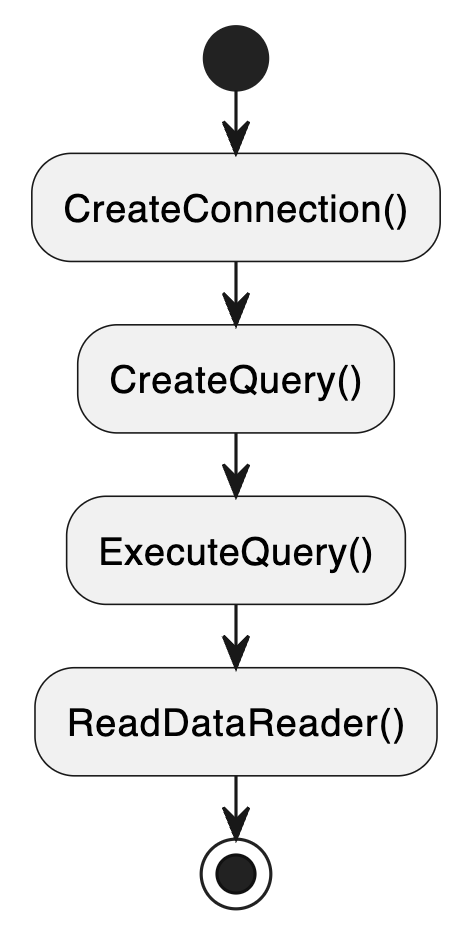
\includegraphics[width=0.3\textwidth]{DatenbankZugriff.png}
      \caption{}
      \label{fig:Datenbankzugriff}
  \end{figure}
\end{center}